% A DUMP OF STUFF THAT WAS IN A DRAFT OF THE PAPER, BUT DIDN'T MAKE THE
% CUT ....



%\todo[inline]{Possible Journals (impact factor in parenthesis) are
%International Journal for Numerical Methods in Fluids (1.6),
%International Journal for Numerical Methods in Engineering (2.1),
%Journal of Scientific Computing (1.9), BIT (1.7), Numerical Mathematics
%Theory Methods and Applications (0.6).  I like International journal for
%Numerical Methods in Fluids which is a Wiley journal}


%We start by assuming that the fluid is governed by the incompressible
%Navier-Stokes equations 
%\begin{align*}
%  \rho\left(\pderiv{\uu}{t} + (\uu \cdot \grad) \uu \right) &= 
%    -\grad p + \mu \Delta \uu \qquad \xx\in\Omega,\\
%    \grad \cdot \uu &= 0 \qquad \xx\in\Omega,
%\end{align*}
%where $\uu$ is the velocity, $p$ is the pressure, $\rho$ is the fluid
%density, and $\mu$ is the fluid viscosity.  The equations are
%nondimensionalized in the standard method which results in the
%dimensionless Reynolds number.  



%\begin{align*}
%  \lim_{\substack{\xx \rightarrow \xx_0 \\ \xx \in \Omega}}
%    \DD[\eeta](\xx) = \UU(\xx_0), \quad \xx_0 \in \Gamma,
%\end{align*}
%for $\eeta$.  When taking the limit, the singularity of the stresslet
%results in a jump~\cite{Pozrikidis1992}, and the density function must
%satisfy  



%When evaluating a target point close to the boundary (as is
%necessary when two particles come close together) the kernel in the
%double layer potential becomes very sharply peaked and thus difficult to
%integrate accurately. Spatial and temporal adaptivity
%\cite{Kropinski1999}, special integration techniques \cite{Klockner2013,
%Ying2006} or asymptotic expansions of lubrication forces
%\cite{Mammoli2006} are all tools that can help, however even if we
%evaluate the double layer potential accurately, time stepping errors can
%still lead to contact. To keep computational costs reasonable we must
%turn to alternative approaches. 

%\begin{figure}[!h]\label{fig:collision_sketch}
%\begin{center}
%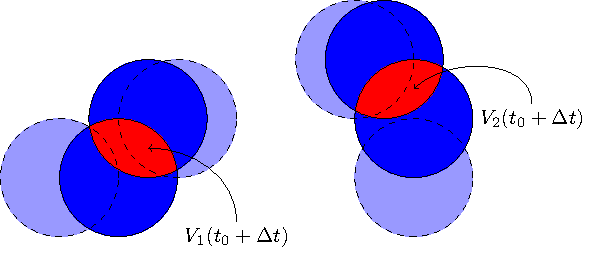
\includegraphics{figures/collisions.pdf}
%\end{center}
%\caption{Sketch of potential collisions.}
%\end{figure}

%Alternatively, repulsion forces can be added~\cite{Malhotra2018}, or
%the analytic solutions of the flow due to lubrication forces can be
%added to the dynamics~\cite{Mammoli2006}.  Unfortunately, repulsion
%forces often introduce non-linear stiffness that restricts the time step
%size, and using lubrication theory is difficult for particles of
%arbitrary geometry due to the complicated asymptotics needed.


%In the BIE setting, computing these quantities is a
%post-processing step, and they are computed with high-order accuracy
%using methods described in Section~\ref{s:method}.

%%%%%%%%%%%%%%%%%%%%%%%%%%%%%%%%%%%%%%%%%%%%%%%%%%%%%%%%%%%%%%%%%%%%%%%%%%%%%%%
%\begin{comment}
%\subsection{Avoiding Contact with STIV}
%Before discussing how collisions can be resolved, we first define a
%metric that measures collision.  This metric should track all pairwise
%collisions and detect if a two particles overlapped not only at the
%discrete time points, but at any time.  We let $\mathbf{V}(t)$ be a
%vector with size $\binom{M_p}{2}$ which is the total number of possible
%pairwise collisions.  $\mathbf{V}$ should be defined in such a way that
%it is 0 if no collisions have occurred, and if there is a collision, its
%value should quantify the amount of overlap.   Then, if there is a
%collision between two particles, the repulsion force should be chosen to
%scale with the magnitude of the corresponding entry of $\mathbf{V}$.
%There are several possible choices for $\mathbf{V}(t)$, the simplest
%being a signed distance between all points on all particles. We use the
%concept of {\em Space-Time Interference Volumes} (STIV) introduced by
%Harmon et al.~\cite{Harmon2011} and adapted for the suspension of
%deformable and rigid particles~\cite{Lu2017}. STIVs involve a time
%integral and are therefore more expensive to compute than other metrics
%(e.g. a signed distance). In most simulations however the cost of
%computing an STIV is dwarfed by the cost of the linear solves necessary
%to compute the velocities of the particles. The advantage of STIVs
%compared to simpler metrics is that under the assumption of ballistic
%motion they are able to detect collisions between two particles that
%pass completely through one another, i.e. it can detect that a collision
%has occurred even if the final candidate configuration is contact-free.
%
%%%%%%%%%%%%%%%%%%%%%%%%%%%%%%%%%%%%%%%%%%%%%%%%%%%%%%%%%%%%%%%%%%%%%%%%%%%%%%%%
%\subsection{Variational Formulation}
%The incompressible Stokes equations can be can be restated as a minimization
%problem. Consider the functional,
%\[ \mathcal{J}(\mathbf{u}) = \int_{\Omega} \nabla\mathbf{u}:\nabla\mathbf{u} -
%2\mathbf{f}\cdot\mathbf{u} ~\text{d}\Omega,\]
%and the associated constrained minimization problem,
%\[ \min \mathcal{J}(\mathbf{u}) ~:~ \nabla\cdot\mathbf{u} = 0 \text{ in
%}\Omega.\]
%Introducing $p$, a Lagrange multiplier for the incompressibility condition, we
%can construct a Lagrangian for this system,
%\begin{equation}\label{eq:lagrangian} \mathcal{L}(\mathbf{u},p) =
%\mathcal{J}(\mathbf{u}) - \int_{\Omega}
%2p\nabla\cdot\mathbf{u}~\text{d}\Omega.\end{equation}
%First order optimality (KKT) conditions for $\mathcal{L}(\mathbf{u},p)$
%recover the incompressible Stokes equations. For our problem, in
%addition to the incompressibility condition, we wish to enforce the
%constraint that the solution $\mathbf{u}$ at a time $t_0$ should not
%introduce collisions at time $t_0+\Delta t$, in other words
%$\mathbf{V}(t_0 + \Delta t) \geq \mathbf{0}$.  This constraint can be
%incorporated in the Lagrangian \eqref{eq:lagrangian} with the
%introduction of a Lagrange multiplier $\llambda$ with one component
%for each possible collision volume,
%\begin{equation}\label{eq:lagrangian2} \tilde{\mathcal{L}}(\mathbf{u},p,\lambda)=
%\mathcal{L}(\mathbf{u},p) + \pmb{\lambda} \cdot \mathbf{V}(t_0+\Delta
%t).\end{equation}
%First order optimality for \eqref{eq:lagrangian2} yields the Stokes equations
%with a modified forcing function,
%\begin{equation}\label{eq:stokes_mod}-\Delta \mathbf{u} + \nabla p = \mathbf{f}%+ \int_{\Omega}
%\text{d}_{\mathbf{u}} \mathbf{V}^T\pmb{\lambda}
%~\text{d}\Omega,\end{equation}
%subject to the constraints
%\[ \nabla\cdot\mathbf{u} =0, ~\mathbf{V}(t_0 + \Delta t) \geq 0,~\pmb{\lambda}
%\geq 0, ~ \pmb{\lambda}\cdot\mathbf{V}(t_0+\Delta t) = 0. \]
%
%The constraints on $\mathbf{V}$ and $\pmb{\lambda}$ can be combined into a
%single constraint,
%\begin{equation}\label{eq:ncp_constraint} \mathbf{V}(t_0 + \Delta t)\geq
%\mathbf{0} \perp \pmb{\lambda}\geq \mathbf{0}.\end{equation}
%
%\end{comment}
%%%%%%%%%%%%%%%%%%%%%%%%%%%%%%%%%%%%%%%%%%%%%%%%%%%%%%%%%%%%%%%%%%%%%%%%%%%%%%%


%%%%%%%%%%%%%%%%%%%%%%%%%%%%%%%%%%%%%%%%%%%%%%%%%%%%%%%%%%%%%%%%%%%%%%%%%%%%%%%%
%\begin{comment}
%\subsection{Complementary Problem}
%
%To compute the repulsion forces we must first compute $\pmb{\lambda}$ for each
%time step such that \eqref{eq:ncp_constraint} is satisfied.
%Consider particles suspended in a fluid in an ambient flow $\mathbf{u}_\infty$.
%This flow can be an imposed background flow or come from solid walls. In the
%later case this velocity field is computed by solving the appropriate resistance problem. In either
%case this flow can be expressed as the sum of a translational component $\mathbf{u}_{\infty}^\tau$,
%a rotational component $\omega_{\infty}$
%and a strain component $\mathbf{e}_{\infty}$,
%\[ \mathbf{u}_{\infty}(\mathbf{x}) = \mathbf{u}_{\infty}^\tau +
%\omega_\infty\times \mathbf{x} + \mathbf{e}_\infty \cdot\mathbf{x}.\]
%The translational and rotational velocity as well as the density
%function of a collection of particles can be computed from the force,
%torque and strain rate~\cite{Karrila1991},
%\begin{equation}\label{eq:mobility} \begin{bmatrix} \mathbf{u}_\infty^\tau -
%\mathbf{u}_\tau\\ \omega^\infty - \omega \\\pmb{\eta}\end{bmatrix} =
%\mathcal{M}\begin{bmatrix}\mathbf{F}\\\mathbf{L}\\\mathbf{e}_\infty\end{bmatrix},\end{equation}
%where $\mathcal{M}$ is the {\em mobility tensor} and depends only on the
%particle configuration $\mathbf{q}^0$ at some time $t^0$. Assuming the
%only force and torques acting on particles arises from repulsion forces,
%we can decompose \eqref{eq:mobility} as,
%\[ \begin{bmatrix} \mathbf{u}_\infty^\tau - \mathbf{u}_\tau\\ \omega^\infty -
%\omega \\\pmb{\eta}\end{bmatrix} =
%\mathcal{M}\begin{bmatrix}\mathbf{0}\\\mathbf{0}\\\mathbf{e}_\infty\end{bmatrix}+
%\mathcal{M}\begin{bmatrix}\mathbf{F}_c\\\mathbf{L}_c\\\mathbf{0}\end{bmatrix}.\]Once
%we solve for $\mathbf{u}_\tau$ and $\omega$ we can update the positions an
%dangles of each particle using an explicit Euler step. With an abuse of
%notation,
%this lets us express a candidate configuration $\mathbf{q}^{1}$ as,
%\[ \mathbf{q}^{1} = \mathbf{q}^n + \Delta
%t\left(\mathcal{M}\begin{bmatrix}\mathbf{0}\\\mathbf{0}\\\mathbf{e}_\infty\end{bmatrix}
%+
%\mathcal{M}\begin{bmatrix}\mathbf{F}_c\\\mathbf{L}_c\\\mathbf{0}\end{bmatrix}\right).\]
%
%This candidate configuration must satisfy the constraint
%\eqref{eq:ncp_constraint}, which we will rewrite to show the dependence of
%$\mathbf{V}$ on both $\mathbf{q}^0$ and $\mathbf{q}^{1}$,
%\begin{equation}\label{eq:ncp_new}\mathbf{V}(\mathbf{q}^0,\mathbf{q}^{1})\geq
%\mathbf{0}\perp \pmb{\lambda}^n\geq \mathbf{0} \Rightarrow
%\mathbf{V}\left(\mathbf{q}^0, \mathbf{q}^0 + \Delta
%t\left(\mathcal{M}\begin{bmatrix}\mathbf{0}\\\mathbf{0}\\\mathbf{e}_\infty\end{bmatrix}
%+
%\mathcal{M}\begin{bmatrix}\mathbf{F}_c\\\mathbf{L}_c\\\mathbf{0}\end{bmatrix}\right)\right)
%\geq \mathbf{0} \perp\pmb{\lambda}\geq \mathbf{0} .\end{equation}
%
%This is a nonlinear complementary problem (NCP). We can see this by explicitly
%including the dependence of $\mathbf{V}$ on $\pmb{\lambda}$,
%\[\mathbf{V}\left(\mathbf{q}^0, \mathbf{q}^0 + \Delta
%t\left(\mathcal{M}\begin{bmatrix}\mathbf{0}\\\mathbf{0}\\\mathbf{e}_\infty\end{bmatrix}
%+ \mathcal{M}\begin{bmatrix} \int_{\Gamma_k}
%\text{d}_\mathbf{u}\mathbf{V}^T\pmb{\lambda}~\text{d}s\\ \int_{\Gamma_k}
%\text{d}_\mathbf{u}\mathbf{V}^T\pmb{\lambda}\cdot(\mathbf{x}-\mathbf{c}_k)^\perp~\text{d}s
%\\\mathbf{0}\end{bmatrix}\right)\right) \geq \mathbf{0} \perp\pmb{\lambda}\geq
%\mathbf{0} .\]
%
%A first order linearization of this NCP turns it into a sequence of linear
%complementary problems (LCP). Starting from an initial guess for
%$\pmb{\lambda}$, $\pmb{\lambda}^0$ the following sequence should converge to the solution of
%\eqref{eq:ncp_new}:
%\begin{equation}\label{eq:lcp}\begin{aligned}
%\mathbf{V}\biggl(\mathbf{q}^0 + \Delta
%t\biggl(\mathcal{M}\begin{bmatrix}\mathbf{0}\\\mathbf{0}\\\mathbf{e}_\infty\end{bmatrix}
%&+ \mathcal{M}\begin{bmatrix} \int_{\Gamma_k}
%\text{d}_\mathbf{u}\mathbf{V}^T\pmb{\lambda}^\ell~\text{d}s\\ \int_{\Gamma_k}
%\text{d}_\mathbf{u}\mathbf{V}^T\pmb{\lambda}^\ell\cdot(\mathbf{x}-\mathbf{c}_k)^\perp~\text{d}s
%\\\mathbf{0}\end{bmatrix}\biggr)\biggr) \\
%&+ \Delta t \mathcal{M}\begin{bmatrix}\int_{\Gamma_k}
%\text{d}_\mathbf{u}\mathbf{V}^T\pmb{\lambda}^{\ell+1}~\text{d}s\\
%\int_{\Gamma_k}
%\text{d}_\mathbf{u}\mathbf{V}^T\pmb{\lambda}^{\ell+1}\cdot(\mathbf{x}-\mathbf{c}_k)^\perp~\text{d}s
%\\\mathbf{0}\end{bmatrix}\frac{\partial\mathbf{V}}{\partial \mathbf{q}^1} \geq
%\mathbf{0} \perp \pmb{\lambda}^{\ell+1} \geq
%\mathbf{0}.\end{aligned}\end{equation}
%
%The sequence \eqref{eq:lcp} will be solved at each time step. 
%\end{comment}
%%%%%%%%%%%%%%%%%%%%%%%%%%%%%%%%%%%%%%%%%%%%%%%%%%%%%%%%%%%%%%%%%%%%%%%





\begin{comment}
\todo[inline]{Do we describe how the preconditioner is updated by simply
rotating?}
After discretizing~\eqref{eqn:bieformulation1}
and~\eqref{eqn:bieformulation2} using the Nystr\"om method, dense linear
systems need to be solved.  The discretized system is solved with
GRMES~\cite{Saad1986}, and since these are both second-kind Fredholm
integral equations, the number of required GMRES iterations is
independent of the resolution~\cite{cam-ips-kel-mey-xue1996}.

with a block diagonal preconditioner and
accelerated using the fast multipole method \cite{Greengard1987}.  Since
the linear system arises from a second kind Fredholm equation the
condition number of the matrix is bounded and does not increase with
finer resolution. The number of GMRES iterations is therefore mesh
resolution independent. This leads to a solver that is $O(n)$, where $n$
is the number of mesh points. 

The matrices described in \eqref{eq:vel_walls} and
\eqref{eq:vel_particles} are full. They can be made block-diagonal by
treating inter-body interactions explicitly and moving them to the
right hand side. This is termed {\em locally implicit} and is described
in \cite{Lu2017}. For dense suspensions however this type of time
stepping can lead to instabilities as bodies become tightly packed. 
\begin{algorithm}
	 \SetKwInOut{Input}{Input}
    	\SetKwInOut{Output}{Output}

  	  \underline{Collision free time stepper}\;
\Input{collision free configuration $\mathbf{q}^0$, time step size $\Delta t$}
\Output{collision free configuration $\mathbf{q}^1$ }
	 $\mathbf{u}^* \gets \mathbf{A}(\mathbf{q}^0,\mathbf{0},\mathbf{0})$\;
	$\mathbf{q}^* \gets \mathbf{q}^0 + \Delta t \mathbf{u}^*$\;
	Compute $\mathbf{V}(\mathbf{q}^0,\mathbf{q}^*)$, $\text{d}_u\mathbf{V}$\;
	\While {$\mathbf{V} < \mathbf{0}$}
	{
		$\llambda \gets$ LCP\_solve($\text{d}_{\mathbf{u}}\mathbf{V}$)\;
$\mathbf{F}_k \gets \int_{\Gamma_k}
\text{d}_{\mathbf{u}}\mathbf{V}^T\llambda~\text{d}s$\;
$L_k \gets \int_{\Gamma_k}
\text{d}_{\mathbf{u}}\mathbf{V}^T\llambda\cdot(\mathbf{x}-\mathbf{c}_k)^\perp~\text{d}s$\;
		$\mathbf{u}^* \gets \mathbf{A}(\mathbf{q}^0,\mathbf{F}_k,\mathbf{L}_k)$\;
		$\mathbf{q}^* \gets \mathbf{q}^0 + \Delta t \mathbf{u}^*$\;
		Compute $\mathbf{V}(\mathbf{q}^0,\mathbf{q}^*)$, $\text{d}_u\mathbf{V}$\;
	}
\end{algorithm}
\end{comment}




%\begin{figure}[!h]
%\begin{center}
%\includegraphics{figures/pressure_contour.pdf}
%\end{center}
%\caption{Pressure distribution inside a Couette device. The outer cylinder is spinning while the
%inner cylinder is fixed. }\label{fig:dissipation}
%\end{figure}






%Mathematically, using STIVs as the collision metric, there is to the
%author's knowledge no theory which guarantees that the LCPs that are
%needed to compute the contact force have a unique solution. This can on
%occasion lead to a non-converging sequence of LCPs. These situations
%appear to be common in suspensions involving solid walls. We have used
%adaptive time-stepping as a way to mitigate this issue, however this is
%entirely heuristic and does not always work. In \cite{Yan2017} a similar
%method is developed that is guaranteed to converge. Instead of using
%STIVs as the collision metric, a signed distance function is used. This
%method, while always convergent, is limited in the sense that it does
%not capture a collision if one body passes completely through another.
%STIVs on the other hand are designed to catch all contact the occurs
%between bodies in a single time step and may be non-zero even if the
%final state is contact-free. 



\begin{comment}
Next, collision detection is
performed.  However, instead of requiring that the bodies are
contact-free, we make the additional restriction that the minimum
separation distance is greater than some user-specified tolerance.
Finally, based on the amount of overlap that occurs, artificial forces
and torques are added to the bodies, and the governing
equations~\eqref{eqn:BIEformulation} are resolved, except that forces
and torques are included in equation~\eqref{eqn:BIEformulation5}.  


To
find the amount of overlap, the space-time interference volume
(STIV)~\cite{Harmon2011} based on a linear trajectory of the rigid
bodies is used. Once the new candidate solution is computed, the
algorithm is repeated until it converges to a contact-free
configuration.
\end{comment}

%At each time step $t^n$ the Stokes equations are solved and the
%particles are advanced to a candidate configuration at $t^{n+1}$.  Using
%a linear interpolant, we check if any collisions occurred in the
%interval $[t^n,t^{n+1}]$.  If the time step is contact-free, the
%candidate configuration is accepted.  If contact is detected, the
%candidate solution is rejected and we resolve
%equations~\eqref{eqn:BIEformulation}, but with artificial repulsion
%forces $\FF^\gamma_j$ and torques $L^\gamma_j$ that are chosen to try
%and avoid contact.  This lets us form a new candidate configuration.
%This process is repeated until we end up with a contact-free
%configuration.



%\begin{comment}
%The addition of a forcing term to the right hand side of the Stokes equations
%would normally lead to a volume integral. However, in this case since
%$\text{d}_{\mathbf{u}} V$ can be non-zero only on the boundary, we can capture
%the repulsion force by adding a net force and torque to each particle or wall as needed. The net
%force $\mathbf{F}^k_p$ and torque $L^k_p$ are given by,
%\[ \mathbf{F}^k_p = \int_{\Gamma_k}
%\text{d}_\mathbf{u}V^T\pmb{\lambda}~\text{d}s, \qquad L_p^k = \int_{\Gamma_k}
%\text{d}_\mathbf{u}V^T\pmb{\lambda}\cdot(\mathbf{x}-\mathbf{c}_k)^\perp~\text{d}s.\]
%\end{comment}



%For example, in the governing equation for the rigid
%bodies~\eqref{eqn:BIEformulation2}, double-layer potential terms is
%discretized as
%\begin{align}
% \DD[\eeta^{N+1}](\xx_j) \approx
%  \DD[\eeta^{N+1}_{k_0}](\xx_j) + 
%  \sum_{\substack{k=1 \\ k \neq k_0}}^{M_p} \DD[\eeta^{N}_k](\xx_j),
%  \label{eqn:BlockImplicit}
%\end{align}
%where $\xx_j$ is on body $k_0$, the superscript denotes the time
%step, and $\DD$ is discretized on the configuration at time step $N$. The interaction between the
%rigid bodies and the solid walls'
%density function, Stokeslets, and rotlets are also discretized
%explicitly.  The advantage of this discretization is that it results in
%a block-diagonal matrix structure that can be solved efficiently by using a block-diagonal
%preconditioner. However, by allowing
%larger interactions between different bodies, stiffness is introduced
%and a smaller time step must be taken. 
%
%Similar to the methodology
%outline described for vesicle suspensions~\cite{Quaife2014}, we instead
%change the fluid solver so that large time steps can still be taken
%without introducing stiffness.  In particular, with the same setup
%described in~\eqref{eqn:BlockImplicit}, we discretize the fluid
%equations as
%\begin{align}
%  \DD[\eeta^{N+1}](\xx_j) = 
%  \sum_{k=1}^{M_p} \DD[\eeta^{N+1}_k](\xx_j).
%  \label{eqn:SemiImplicit}
%\end{align}
%Equation~\eqref{eqn:SemiImplicit} is no longer block-diagonal and requires additional computational
%resources. In particular
%interactions between different bodies must be computed at every
%iteration rather than once per time step (to form the right hand side).
%However, as was observed for dense vesicle suspensions~\cite{Quaife2014, Rahimian2015} this
%additional cost is offset by the
%excessively small time step that is required if the fluid
%solver~\eqref{eqn:BlockImplicit} is used.  Moreover, as we will see in
%the Results section, it is possible that if the buffer region is
%sufficiently small and the suspension is sufficiently dense,
%then~\eqref{eqn:BlockImplicit} is unstable for time step sizes that vary
%over several orders of magnitude.





